\chapter{実装}
\label{chap:zisso}

%ーーーーーーーーーーーーーーーーーーーーーーーーーーーー

\section{実装環境}
本研究での実装環境は下記である. 

\begin{itemize}
 \item オペレーティングシステム
    \begin{itemize}
      \item Mac OS Ventura 13.4.1
    \end{itemize}
 \item 実装言語
    \begin{itemize}
      \item Python 3.11.6
    \end{itemize}
\end{itemize}

%ーーーーーーーーーーーーーーーーーーーーーーーーーーーー

\section{Google Playストアのスクレイピング}
本研究で取得するレビュー情報は先行研究\cite{kawatsura}に合わせて下記とする. 

\begin{itemize}
 \item reviewId : レビューID
 \item userName : ユーザ名
 \item userImage : ユーザのプロフィール画像
 \item at : 投稿日時
 \item score : 星の数
 \item content : レビュー内容
 \item thumbsUpCount : このレビューが参考になったと評価した人の数
 \item reviewCreatedVersion : レビュー時のバージョン
 \item replyContent : 開発者からの返信の内容
 \item repliedAt : 開発者からの返信日時
\end{itemize}

先行研究では投稿日時が2021年10月21日〜2021年12月15日までの8週間のレビューを収集している. 収集されたGoogle Playストアの各アプリのレビュー数は表\ref{tb:rawreviewnum}の通りである. 
\begin{table}[htbp]
  \caption{収集したGoogle Playストアのレビュー数(2021/10/21〜12/15)(\cite{kawatsura} p.16, 表 4.2)}
  \label{tb:rawreviewnum}
  \begin{center}
  \begin{tabular}{l|l}
    \hline
    アプリ名&収集したレビュー数(件)\\\hline\hline
    にゃんトーク&171\\\hline
    スマートニュース&1,651\\\hline
    PayPay&1,052\\\hline
    Coke ON&1,736\\\hline
    Google Fit&372\\\hline
    Simeji&468\\\hline
    Lemon8&72\\\hline
    楽天ペイ&480\\\hline
    majica&706\\\hline
    LINE MUSIC&359\\\hline
    BuzzVideo&375\\\hline
    ファミマのアプリ&290\\\hline
    CapCut&180\\\hline\hline
    合計&7,912
  \end{tabular}\end{center}
\end{table}

この先行研究のデータに加え, 本研究では2023年10月1日〜12月15日のレビューを新たに取得する. 新たに取得されたGoogle Playストアの各アプリのレビュー数は表\ref{tb:rawreviewnum2023}の通りである. 
\begin{table}[htbp]
  \caption{収集したGoogle Playストアのレビュー数(2023/10/1〜12/15)}
  \label{tb:rawreviewnum2023}
  \begin{center}
  \begin{tabular}{l|l}
    \hline
    アプリ名&収集したレビュー数(件)\\\hline\hline
    にゃんトーク&\\\hline
    スマートニュース&\\\hline
    PayPay&\\\hline
    Coke ON&\\\hline
    Google Fit&\\\hline
    Simeji&\\\hline
    Lemon8&\\\hline
    楽天ペイ&\\\hline
    majica&\\\hline
    LINE MUSIC&\\\hline
    ファミマのアプリ&\\\hline
    CapCut&\\\hline\hline
    合計&
  \end{tabular}\end{center}
\end{table}

Google PlayストアのレビューをスクレイピングするためにPythonのプログラムである(\verb|get_google_play_review.py|)を作成した. このプログラムの作成にあたり, Pythonのライブラリであるgoogle-play-scraperを使用する. google-play-scraperでは外部依存関係なしでPython用のGoogle Playストアを簡単にクロールするためのAPIが提供されている\cite{google-play-scraper}. 
このライブラリを使用することにより, アプリのパッケージ名, 言語, 取得する数, 順序を指定してレビューの一覧を取得することができる. 

%ーーーーーーーーーーーーーーーーーーーーーーーーーーーー

\section{Xのスクレイピング}
\label{sec:x}
本研究で取得するツイート情報は先行研究\cite{kawatsura}に合わせて下記とする. 
\begin{itemize}
 \item id : ツイートID
 \item content : ツイート内容
 \item at : ツイート日時
\end{itemize}

先行研究では投稿日時が2021年10月21日〜2021年12月15日までの8週間のツイートを収集している. 収集されたTwitterの各アプリのツイート数を表\ref{tb:rawtweetnum}に示す. 

\begin{table}[htbp]
  \caption{収集したTwitterのツイート数(2021/10/21〜12/15)(\cite{kawatsura} p.18, 表 4.3)}
  \label{tb:rawtweetnum}
  \begin{center}
  \begin{tabular}{l|l}
    \hline
    アプリ名&収集したツイート数(件)\\\hline\hline
    にゃんトーク&2,525\\\hline
    スマートニュース&50,590\\\hline
    PayPay&880,319\\\hline
    Coke ON&84,424\\\hline
    Google Fit&13,496\\\hline
    Simeji&205,327\\\hline
    Lemon8&4,376\\\hline
    楽天ペイ&11,111\\\hline
    majica&3,649\\\hline
    LINE MUSIC&184,873\\\hline
    BuzzVideo&41,656\\\hline
    ファミマのアプリ&8,867\\\hline
    CapCut&33,998\\\hline\hline
    合計&1,525,211
  \end{tabular}\end{center}
\end{table}

この先行研究に加え, 本研究では新たに2023年10月〜12月のポストを取得する. Xのポスト取得に関してはTwitter APIを使用してスクレイピングを行う. Twitter APIのプランに関してはFree, Basic, Pro, Enterpriseの4つのプランが用意されておりそれぞれ料金や使用できる機能などが異なる. 大規模なサービスやビジネス向けのEnterpriseプラン以外の3つのプランの違いの一部を表\ref{tb:xplan}に示す. 
表\ref{tb:xplan}よりポストを取得するためにはBasicプラン以上に加入する必要がある. Basicプランに加入した場合でも合計で30,000件しか取得されないため本研究では先行研究のデータセットを追加で使用することとした. Xの利用規約によると, Xが提供するインターフェイスを介して行うスクレイピング以外は禁止としている. そのため, seleniumなどを使用したスクレイピングはせずに, 先行研究のデータを使用することとした. 

\begin{table}[htbp]
  \caption{プランとできること}
  \label{tb:xplan}
  \begin{center}
  \begin{tabular}{|l|c|c|c|}
    \hline
    &Free&Basic&Pro \\\hline\hline
    料金&無料&月額100ドル&月額5,000ドル \\\hline
    月間ポスト数の上限&1,500&3,000&300,000 \\\hline
    月間ポスト取得数&0&10,000&1,000,000 \\\hline
  \end{tabular}\end{center}
\end{table}

Twitter APIを使用してポストを取得するためにPythonのプログラムである(\verb|get_tweet.py|)を作成した. このプログラムではTwitter APIにアクセスするためのライブラリであるTweepy\cite{tweepy}を使用した. まずAPIキーなどの4つの認証情報をセットする. 次にClientクラスのsearch\_resent\_tweetメソッドを使用してツイートを取得する. 
このメソッドは最大で過去7日間まで遡ってツイートを取得できる. search\_all\_tweetsメソッドでは全てのツイートを取得できるが, ``Academic Research''という学術用の用途でAPI承認されたユーザーしか使用できないため本研究では使用しなかった. 
先行研究と同じ情報を取得するために, 本研究では引数として以下のものを与えた. 
\begin{itemize}
 \item max\_resul : 検索結果の最大数. 10〜100の数値で, デフォルトは10
 \item query: 検索ワード
 \item tweet\_field: ツイートフィールドを選択. 今回はツイート日時を取得するために["created\_at"]とした. 
 \item end\_time: 期間の終わりを指定できる(UTCタイムスタンプ)
\end{itemize}

新たに取得したXのポスト数を表\ref{tb:rawtweetnum2023}に示す

\begin{table}[htbp]
  \caption{収集したXのポスト数(2023年10月〜2023年12月)}
  \label{tb:rawtweetnum2023}
  \begin{center}
  \begin{tabular}{l|l}
    \hline
    アプリ名&収集したツイート数(件)\\\hline\hline
    にゃんトーク&\\\hline
    スマートニュース&\\\hline
    PayPay&\\\hline
    Coke ON&\\\hline
    Google Fit&\\\hline
    Simeji&\\\hline
    Lemon8&\\\hline
    楽天ペイ&\\\hline
    majica&\\\hline
    LINE MUSIC&\\\hline
    ファミマのアプリ&\\\hline
    CapCut&\\\hline\hline
    合計&
  \end{tabular}\end{center}
\end{table}

%ーーーーーーーーーーーーーーーーーーーーーーーーーーーー

\section{前処理}
機械学習によるレビューに含まれる有用な箇所の自動抽出における精度を上げるために, GooglePlayストアとXから取得したデータに対して前処理を行うプログラム(\verb|preprocessing_google.py|, \verb|preprocessing_twitter.py|)を作成した. この処理では以下に示す処理を行う. この処理は一般的な自然言語処理の手法を参考としている. 
\begin{itemize}
  \item 英語を全て小文字に揃える. 
  \item 以下の文字列を削除. 
    \begin{itemize}
      \item 「」【】()()『』
      \item @@から始まるメンション
      \item \#から始まるタグ
      \item URL
      \item 半角空白,全角空白
      \item 絵文字
      \item 日本語を含まないレビュー
    \end{itemize}
  \item レビューやツイートには, 異なる欠陥の報告やアプリに対する要望に関する文が2文以上からなるものがある. そのため, 「。」「.」「!」「!」「?」「!」「\verb|\n|」「\verb|\r\n|」でそれぞれの文に分割する. 
\end{itemize}
以下の図\ref{chap:preprocessing}がレビューを前処理した例である. 2つの文で構成されているため「。」で区切り分割している. また絵文字は削除されている. 

\begin{figure}[hbtp]
 \centering
 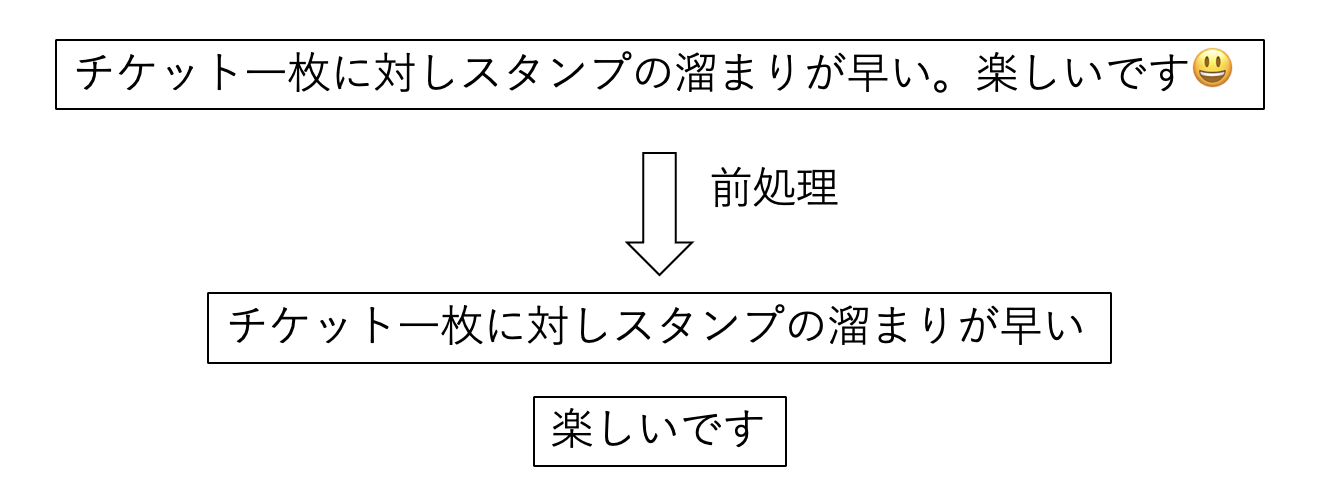
\includegraphics[scale=0.5]
      {contents/images/preprocessing.png}
 \caption{前処理の例\label{chap:preprocessing}}
\end{figure}

前処理した結果をcsvファイルにて保存する. 保存する項目としては, 投稿日時(at), レビューのid(reviewId)またはツイートid(id), そして, 前処理した文章である. 図\ref{tb:googlecsv}, 図\ref{tb:twittercsv}に前処理結果後のcsvファイルの一部を示す. 

\begin{table}[htbp]
  \caption{Google Playストアレビューの前処理結果(buzzvideo)}
  \label{tb:googlecsv}
  \begin{center}
  \begin{tabularx}{\linewidth}{|l|l|X|}
    \hline
    at&reviewId&content\\\hline\hline
    2021-12-15 19:25:30&gp:AOqpTOHj6w ...&バズビデオを見て、感動をありがとう\\\hline
    2021-12-15 12:28:09&gp:AOqpTOHleV ...&内容が残酷で異常な人が多い\\\hline
    2021-12-15 11:09:50&gp:AOqpTOHG7O ...&分かりづらい\\\hline
    2021-12-14 15:16:33&gp:AOqpTOGWvT ...&ばず29さいって人が投稿してる動画すべて虚偽動画なのでアカウント削除と動画削除して欲しい\\\hline
    2021-12-14 15:16:33&gp:AOqpTOGWvT ...&あるだけで大迷惑です\\\hline
    2021-12-14 15:16:33&gp:AOqpTOGWvT ...&二度と登録し直せないよう個体識別番号で縛ってください\\\hline
    2021-12-14 15:16:33&gp:AOqpTOGWvT ...&お願いします\\\hline
  \end{tabularx}\end{center}
\end{table}

\begin{table}[htbp]
  \caption{ツイートの前処理結果(BuzzVideo)}
  \label{tb:twittercsv}
  \begin{center}
  \begin{tabularx}{\linewidth}{|l|l|X|}
    \hline
    at&id&content\\\hline\hline
    2021-12-15T23:55:11.000Z&1471267626655825922&芸能人に似てる気がするけど名前が思い出せない\\\hline
    2021-12-15T23:53:43.000Z&1471267256659509249&驚愕男性が豆乳を飲むべき3つの理由\\\hline
    2021-12-15T23:53:43.000Z&1471267256659509249&男だからこそ注目したい豆乳のメリットとは\\\hline
    2021-12-15T23:53:17.000Z&1471267149746679813&感情を乗せた歌声と歌詞に聞き惚れちゃう♪壊れかけのradio\\\hline
    2021-12-15T23:53:10.000Z&1471267120264904705&kkと眞子の酷い嘘\\\hline
    2021-12-15T23:53:10.000Z&1471267120264904705&恐ろしい真実が明らかに\\\hline
  \end{tabularx}\end{center}
\end{table}

%ーーーーーーーーーーーーーーーーーーーーーーーーーーーー

\section{有用な箇所の自動抽出}
\subsection{データセット}
モデルのfine-tuningに使用されるデータセットとして, Google PlayストアとXのツイートからそれぞれ5,000件ずつ合計で10,000件のデータをランダムに抽出し手作業で有用な箇所を抽出した. データセットの作成は情報工学科の学部4年生2人がそれぞれ手作業で行い, お互いの抽出した箇所が異なっていたものは議論することにより統一した. 
データセットには前処理したデータが格納されたcsvファイルを利用して, 抽出したオブジェクトを含めた新たなcsvファイルを作成する. 作成されたcsvファイルにはid,アプリ名,投稿日時,本文, 抽出したオブジェクトの5つのデータが入っている. idは前処理したデータを識別するために与えられ, Google Playストアのレビュー文はg\_(index), twitterのツイートのidはt\_(index)とする.  indexには各データに応じた番号が振られている. 
10,000件のデータセットのうち, 6,000件を訓練データ, 2,000件を検証用データ, 2,000件をテストデータとする. 質問応答形式のfine-tuningを行うために, csv形式であるデータセットをソースコード\ref{json}に示すようにjson形式に変換する. 

\begin{lstlisting}[caption=データセット.json,label=json]
  {
    "version": "v2.0", 
    "data": [
      {
        "title": "モバイルアプリのレビュー", 
        "paragraphs": [
          {
            "context": "本アカウントのフォローやリツイートお願いします",
            "qas": [
              {
                "id": "t_2223388",
                "question": "この文はTwitterのツイートです。
                             paypayアプリの欠陥やpaypayアプリに対する
                             要望が書かれているのはどこですか?",
                "is_impossible": true,
                "plausible_answers": [{"text": "", "answer_start": -1}],
                "answers": [{"text": "", "answer_start": -1}]
              }
            ]
          },
          {
            "context": "11/25前後からアプリを開いても強制終了、
                      会員バーコードもクーポンも何も出せない状態、
                      これでは買い物ができないと、こちらのレビュー
                      を見に来て沢山の方が同じ状態であることが
                      わかった",
            "qas": [
              {
                "id": "g_6041", 
                "question": "この文章はGooglePlayストアのレビューです。
                            majicaアプリの欠陥やmajicaアプリに対する
                            要望が書かれているのはどこですか?",
                "answers": [{"text": "アプリを開いても強制終了、
                                      会員バーコードもクーポン
                                      も何も出せない", 
                             "answer_start": -1}], 
                "is_impossible": false
              }
            ]
          }, ...
        ]
      }
    ]
  } 
\end{lstlisting}

このjsonファイルは下記の要素によって構成になっている. 

\begin{itemize}
  \item version: バージョンを表す. 今回は答えられない質問を含むSQuAD 2.0と同じバージョンのため, v2.0とする
  \item title: contextのタイトル
  \item paragraphs: context1つとそれに関連する質問, 答えがリスト形式で保持されている
  \item qas: 質問と回答がリスト形式となっている
  \item context: 元の文章(抽出する前の文章)
  \item id: 設定したid
  \item question: 質問文
  \item is\_impossible: 答えられない質問ならtrue, それ以外はfalse
  \item plausible\_answers: 質問が答えられない時のみ存在し, 問題文から答えになりうる部分を抽出
  \item answers: contextから抜き出した答えとその位置情報がリスト形式で保持されている. 答えを複数用意することもできる. 
  \item text: contextから抜き出した答えのテキスト情報(抽出する文章)
  \item answe\_start: contextから抜き出した答えの位置情報
\end{itemize}

\subsection{モデルのfine-tuning}
用意したデータセットを用いて事前学習済みモデルをfine-tuningする. 本研究では事前学習済みモデルとしてHuging FaceのTransformersを通して利用できる東北大学のモデル\cite{tohoku}を使用する. このモデルは日本語のWikipediaのデータを用いて学習されている\cite{tohoku}. 
この東北大学が公開している日本語BERTのうち, whole word maskingを適用して学習させているモデル\cite{masking}を用いる. whole word maskingとは事前学習時に単語ごとでマスクするかどうかを決め, マスクする単語に対応するサブワードを全てマスクする方式である. モデルのパラメータは以下に示す通りである. 
\begin{itemize}
  \item 学習率: 3e-5
  \item エポック数: 10
  \item バッチサイズ: 12
\end{itemize}

実装にはTransformersに含まれるスクリプトであるrun\_squad.pyを用いる. 

\subsection{自動抽出}
fine-tuningを行ったモデルを使用して自動抽出を行う. 前処理したGooglePlayストアのデータと, twitterのデータから有用な箇所を自動抽出する. 

結果は表\ref{tb:googleqa}に示すようにcsv形式で保存する. 

\begin{table}[htbp]
  \caption{Google Playストアレビューの自動抽出結果(google\_fit)}
  \label{tb:googleqa}
  \small
  \begin{center}
  \begin{tabularx}{\linewidth}{|l|l|X|X|X|}
    \hline
    id&app\_name&datetime&context&prediction\\\hline\hline
    g\_955&coke\_on&2021-11-27 11:17:03&商品が出ない事が何回か発生しました&商品が出ない\\\hline
    g\_956&coke\_on&2021-11-02 12:15:37&使用している端末が、利用できる端末の一覧表にないため、サポートは期待できない&使用している端末が、利用できる端末の一覧表にない\\\hline
    g\_959&coke\_on&2021-11-11 15:32:50&そもそも自販機側が黄色点滅していなくて買えないことが多過ぎです&自販機側が黄色点滅していなくて買えない\\\hline
    g\_961&coke\_on&2021-11-14 23:13:26&今まではcoke\_on対応を優先してかっていたが、これからはコカコーラ製品全般をできるだけ買わないようにする&今まではcoke\_on対応を優先してかっていたが、これからはコカコーラ製品全般をできるだけ買わないようにする\\\hline
    g\_964&coke\_on&2021-10-24 12:30:07&自販機との接続を早くしてほしい&自販機との接続を早くしてほしい\\\hline
    g\_965&coke\_on&2021-11-11 16:43:39&やっと繋がっても先にキャンペーン広告が出てすぐに買えないのが不親切&キャンペーン広告が出てすぐに買えない\\\hline
    g\_969&coke\_on&2021-12-07 08:28:27&コークオンパスのフリー20プランの残り回数が分かりやすく表示してほしい&コークオンパスのフリー20プランの残り回数が分かりやすく表示してほしい\\\hline
    g\_973&coke\_on&2021-11-23 14:51:45&反応しない&反応しない\\\hline
    g\_977&coke\_on&2021-11-11 18:22:04&2本以上の購入はとても使えません&2本以上の購入はとても使えません\\\hline
    g\_978&coke\_on&2021-11-01 11:06:09&それと対応自販機との連携が悪い&自販機との連携が悪い\\\hline
    g\_980&coke\_on&2021-10-22 03:22:06&動きが遅い&動きが遅い\\\hline
    g\_982&coke\_on&2021-11-22 11:58:45&ただ自分のスマホのストレージが小さく、データ容量が大きいため今回一先ず削除いたします&自分のスマホのストレージが小さく、データ容量が大きい\\\hline
  \end{tabularx}\end{center}
\end{table}

%ーーーーーーーーーーーーーーーーーーーーーーーーーーーー

\section{クラスタリング}
\subsection{ベクトルの生成}
抽出した文章をその文章が示す意味に応じてクラスタリングする. クラスタリングするために日本語Sentence-BERTクラスを定義する. 日本語Sentence-BERTクラス(SentenceBertJapanese)の各関数の概要を示す. 
\begin{itemize}
  \item \_\_init\_\_関数 : モデルとトークナイザーの初期化を行う. 
  \item \_mean\_pooling関数 : モデルの出力とAttention Maskを用いて, 文の埋め込みを生成するための平均プーリングを行う
  \item encode関数 : 文のリストから各文章の埋め込みを求める. 
\end{itemize}

このように, 日本語のBERT用に転移学習したBERTを用いて各トークンの埋め込みを求め, 平均を取ることにより文全体の埋め込みを求めている. 

% \begin{lstlisting}[caption=clustering.py,label=sentence-bert]
%   class SentenceBertJapanese:
%     def __init__(self, model_name_or_path, device=None):
%         self.tokenizer = BertJapaneseTokenizer.from_pretrained(model_name_or_path)
%         self.model = BertModel.from_pretrained(model_name_or_path)
%         self.model.eval()

%         if device is None:
%             device = "cuda" if torch.cuda.is_available() else "cpu"
%         self.device = torch.device(device)
%         self.model.to(device)

%     def _mean_pooling(self, model_output, attention_mask):
%         token_embeddings = model_output[0] #First element of model_output contains all token embeddings
%         input_mask_expanded = attention_mask.unsqueeze(-1).expand(token_embeddings.size()).float()
%         return torch.sum(token_embeddings * input_mask_expanded, 1) / torch.clamp(input_mask_expanded.sum(1), min=1e-9)

%     @torch.no_grad()
%     def encode(self, sentences, batch_size=8):
%         all_embeddings = []
%         iterator = range(0, len(sentences), batch_size)
%         for batch_idx in iterator:
%             batch = sentences[batch_idx:batch_idx + batch_size]

%             encoded_input = self.tokenizer.batch_encode_plus(batch, padding="longest", 
%                                            truncation=True, return_tensors="pt").to(self.device)
%             model_output = self.model(**encoded_input)
%             sentence_embeddings = self._mean_pooling(model_output, encoded_input["attention_mask"]).to('cpu')

%             all_embeddings.extend(sentence_embeddings)

%         # return torch.stack(all_embeddings).numpy()
%         return torch.stack(all_embeddings)
% \end{lstlisting}

SentenceBertJapaneseクラスの引数に日本語モデル名を与えることによりインスタンスが生成され, モデルの読み込みが完了する. このインスタンスを使用して抽出されたオブジェクトをベクトルに変換する. 

% \begin{lstlisting}[caption=clustering.py,label=model]
%   model = SentenceBertJapanese("sonoisa/sentence-bert-base-ja-mean-tokens")
% \end{lstlisting}

\subsection{グラフクラスタリング}
次に, それぞれの抽出したオブジェクトをノード, ノードのベクトル間のコサイン類似度をエッジとする無向グラフを作成する. 作成されたグラフからChinese Whispersによりグラフクラスタリングが実行される. 
クラスタリングした結果, それぞれの文章にクラスタの番号(以下 : クラスタ番号)が振られ, クラスタ番号が同じものが同じクラスタとなり番号が近いものは意味的相関が近いことを表す. コサイン類似度の閾値を決めることによりどの程度の類似文を同じクラスタと定義するのかが決定される. 本研究では検証を重ねた結果, 閾値は0.8とした. 
結果はcsvファイルに保存される. 表\ref{tb:clustering}に示されるように抽出した文章にクラスタ番号が振られる. 

\begin{table}[htbp]
  \caption{抽出した文章とクラスタ番号(google\_fit)}
  \label{tb:clustering}
  \begin{center}
  \begin{tabularx}{\linewidth}{|X|c|}
    \hline
    prediction&cluster\\\hline\hline
    十分歩いて108歩とかふざけんな&273\\\hline
    278歩に減っていた&274\\\hline
    再起動しても直らない&275\\\hline
    接続/連携を適宜確認しておく必要がある&276\\\hline
    歩いた歩数より足りない&279\\\hline
    使えない&280\\\hline
    使えない&280\\\hline
    歩けない&280\\\hline
    使えない&280\\\hline
    動かなかった&280\\\hline
    反応しない&280\\\hline
    使い方も分からない&280\\\hline
    使えない&280\\\hline
    使えない&280\\\hline
    動かなくなった&280\\\hline
    長期放置されてるんでしょうか&281\\\hline
    下がるって何故でしょうか&282\\\hline
    カウントされなくなる&283\\\hline
    何もカウントしなくなった&283\\\hline
    カウント出来ていない&283\\\hline
    カウントされず&283\\\hline
    記録ができませんと&283\\\hline
    計測しなくなった&283\\\hline
    カウントされなくなった&283\\\hline
    カウントしない&283\\\hline
    全くカウントされていない&283\\\hline
    カウントしなくなりました&283\\\hline
    データが反映されなくなった&283\\\hline
  \end{tabularx}\end{center}
\end{table}

\subsection{クラスタのタイトル}
クラスタのタイトルの決定には, MultipartieRankを使用したキーワード抽出を利用する. 実装にはpke(python keyphrase extraction)というキーワード抽出ライブラリを使用する. 
抽出するための手法や対象となる言語, 抽出する品詞を指定することができる. 


%ーーーーーーーーーーーーーーーーーーーーーーーーーーーー

\section{画面出力・可視化}
\subsection{使用した言語・フレームワーク}
webアプリケーションの実装に使用した言語, フレームワークは以下となっている. 
\begin{itemize}
    \item フロントエンド: HTML/CSS, JavaScript
    \item バックエンド: Python
    \item フレームワーク: Flask
\end{itemize}

\subsection{概要}
分類した結果の含まれたcsvファイルの情報をバックエンド側で処理し, リストを作成する. そのリストをフロントエンド側に渡し処理することでレビューの情報をwebブラウザ上に表示することができる. 

\subsection{画面構成}
画面は大きく分けて一覧画面とアプリごとの詳細画面の2つである. 

一覧画面では全てのアプリに対する日ごとのレビュー数を表す折れ線グラフを表示する. 
このグラフをGoogle Playストアのレビューとツイートの2つ作成する. 

アプリごとの詳細画面では, アコーディオンメニューを使用して抽出した文章の一覧をクラスタごとに表示する. また, 抽出した文章をクリックすると投稿日時や元のレビュー文がモーダルウィンドウで表示する. 
そして, 日ごとのレビュー数を表す折れ線グラフとクラスタに含まれるレビュー数の上位10個を表す棒グラフの2つのグラフを表示する. 

\subsection{検索のロジック}
検索項目である期間とキーワードを指定するとその情報がバックエンド側に渡され, 処理することでリストを更新する. 更新されたリストの情報をフロント側に渡すことで検索結果が反映される. 
ツイートのリストを検索結果に応じて更新するソースコード\ref{search}を示す. 

\begin{lstlisting}[caption=view.py, label=search]
  # ファイル読み込み, 日付でソートしたリスト作成
  with open('該当アプリのcsvファイルの相対パス', 'r', encoding='utf-8-sig') as csv_file:
      csv_reader = csv.reader(csv_file)
      rows = list(csv_reader)
      rows = sorted(rows, reverse=False, key=lambda x:x[2])

  # 検索結果のリスト作成
  search_result = []
  for row in rows:
      if start_date <= row[2][:10] <= end_date:
          if keyword != '':
              if keyword in row[3]:
                  search_result.append(row)
          else:
              search_result.append(row)
  rows = search_result
\end{lstlisting}

% アルゴリズム
% \begin{figure}[!t]
%   \begin{algorithm}[H]
%       \caption{Search}
%       \label{search}
%       \begin{algorithmic}[1]
%         \STATE $path \leftarrow$ '../クラスタリング/twitter\_\{app\_name\}.csv'
%         \STATE Open $twitter\_csv\_file$ with encoding 'utf-8-sig'
%         \STATE $twitter\_csv\_reader \leftarrow$ CSV reader for $twitter\_csv\_file$
%         \STATE $twitter\_rows \leftarrow$ Convert $twitter\_csv\_reader$ to a list
%         \STATE Sort $twitter\_rows$ in ascending order by the date (element at index 2)
%         \STATE $search\_result \leftarrow$ Empty list
%         \FOR{$row$ in $twitter\_rows$}
%           \IF{$start\_date \leq row[2][:10] \leq end\_date$}
%             \IF{$keyword \neq ''$}
%               \IF{$keyword$ is in $row[3]$}
%                 \STATE Append $row$ to $search\_result$
%               \ENDIF
%             \ELSE
%               \STATE Append $row$ to $search\_result$
%             \ENDIF
%           \ENDIF
%         \ENDFOR
%         \STATE $twitter\_rows \leftarrow search\_result$
%       \end{algorithmic}
%   \end{algorithm}
% \end{figure}

\subsection{グラフの作成}
グラフの作成にはplotly.js\cite{plotly}を用いる. plotly.sjとはグラフ生成ライブラリであり, 3Dグラフや統計グラフなど40を超えるグラフタイプが同梱されている\cite{plotly}.
plotly.jsで作成されたグラフにはオプションとしてズーム機能やグラフのダウンロード機能が付随している. 
日付ごとのレビュー数に関するグラフを表示するソースコード\ref{graph}を示す. 設定したタグをDOMのターゲットにしてplotly.jsに書き換えてもらう. graphsはバックエンド側で作成された日付とその日のレビュー数に関する二次元リストであり, 横軸に日付, 縦軸にレビュー数を取るグラフである. 
dataのtypeでグラフタイプを指定でき, layoutでタイトルや表の大きさを指定できる. 

\begin{lstlisting}[caption=detail.html, label=graph]
  <div class="graph-title">日付ごとのレビュー数の推移</div>
  <div id="scatter"></div>

  <script>
      // 横軸: 日付
      var labels = JSON.parse('{{ graphs | map(attribute=0) | list | tojson | safe }}');
      // ラベル用日付
      var displayLabels = [];
      for (var i = 0; i < labels.length; i += 5) {
          displayLabels.push(labels[i]);
      }
      var values = JSON.parse('{{ graphs | map(attribute=1) | list | tojson | safe }}');

      var data = [{
          x: labels,
          y: values,
          type: 'scatter',
      }];

      var layout = {
          title: '日付ごとのレビュー数の推移',
          height: 600,
          width: 1200,
          xaxis: {
              tickvals: displayLabels,  // 配列の5つおきの目盛り位置を指定
          }
      };

      Plotly.newPlot('scatter', data, layout);
  </script>
\end{lstlisting}


